The conditioning process, consisting of cleaving and polishing the fibers, is an individual task that generates a small dispersion in the response of each individual fiber, $\sigma_{con}$. This uncertainty is present in the tritium measurement by the monitor. To measure this uncertainty, it has to be taken into account that the position of the connectors that lock the fiber in the experimental setup produce an additional uncertainty, $\sigma_{pos}$, in the measurement. Since both uncertainties are independent, the total uncertainty is given by:

\begin{equation}
\sigma_{t} = \sqrt{\sigma^2_{pos} + \sigma^2_{con} }
\label{eq:TotalUncertaintyFiberCharacterization}
\end{equation}
The uncertainty due to the fiber position has to be quantified to extract the conditioning uncertainty from the total uncertainty. Two different experiments were designed, the first giving only the uncertainty in the fiber position ($\sigma_{t} = \sigma_{pos}$), and the second to obtain the total uncertainty. The conditioning uncertainty is given by,

\begin{equation}
\sigma_{con} = \sqrt{\sigma^2_{tot} - \sigma^2_{pos} }
\label{eq:ConditioningUncertaintyFiberCharacterization}
\end{equation}
The test designed to measure $\sigma_{pos}$ consisted of preparing one fiber of each type (uncladded, single clad and multiclad) by the conditioning process reported above. Each fiber was locked in the setup, and measurements by feeding the LED with an intensity of $0.1~\milli\ampere$  are made. These measurements were repeated ten times with a given fiber. The mean, $\bar{x}$, and the standard deviation of the measurements for each fiber type are shown in Table \ref{tab:PositionStandardDeviation} where the relative standard deviation, $\sigma^{rel}_{pos}$, defined by equation \ref{eq:RelativeStandardDesviation}, is also included.

\begin{equation}
\sigma^{rel}_{pos} = \frac{\sigma_{pos}}{\bar{x}}
\label{eq:RelativeStandardDesviation}
\end{equation}

\begin{table}[htbp]
\centering{}%
\begin{tabular}{lccc}
\toprule 
Fiber type & Mean ($\text{photons}$/ns) & $\sigma_{pos}$ ($\text{photons}$/ns) & $\sigma^{rel}_{pos}$ (\%) \tabularnewline
\midrule
\midrule 
Uncladded & $524.09 \pm 0.01$ & $17.65$ & $3.37$ \tabularnewline
Single Clad & $1071.70 \pm 0.01$ & $9.07$ & $0.85$ \tabularnewline
Multiclad & $949.93 \pm 0.03$ & $9.91$ & $1.04$ \tabularnewline
\bottomrule
\end{tabular}
\caption{Mean and standard deviation (due to fiber position in the setup) of photons per nanosecond that reach the PMT for $0.1~\milli\ampere$ LED intensity.}
\label{tab:PositionStandardDeviation}
\end{table}
As it can be noticed, the clad reduces the position uncertainty, which means that it improves the uniformity of the fiber response. It was also found that the clad significantly improves the light collection efficiency of the fibers. The reason could be that photons are mainly collected in the core of the fiber and the interface of core is better defined for single-clad and multi-clad fibers than for uncladded fibers. In the latter case, the interface is provided by the environment (air or water in the case of TRITIUM). External conditions, as dirt, may produce noticeable interface fluctuations. It is also seen in the table that a second clad slightly reduce the collection efficienciy. The reason could be that a second clad layer reduces the radious of the fiber core proportionally. Concerning the error of the measurement, the error of the Keithley device was three orders of magnitude smaller than the standard deviation of the measurement and was neglected.

%In addition to the $\sigma_{pos}$ measurement, we have measured the number of photons collected by each type of fiber in the same situation, which is higher for single clad and even higher for multiclad. It means that the clad has an appreciable effect on the fiber collection efficiency and it could be a possible point to futur studies.

To determinate the whole uncertainty, ten different samples of each fiber type were prepared and each fiber was measured under the same conditions as above. This measurement was done for four different LED emission intensities ($0.05$, $0.1$, $0.15$ and $0.2~\milli\ampere$). The results for uncladded fibers are plotted in Figure \ref{fig:10samplesNC}, where it can be seen that, although each fiber shows a very linear trend with the number of collected photons, a dispersion in the fiber response is clearly seen. Similar results were obtained for single clad and multiclad fibers, displayed in figures \ref{subfig:10samplesSC} and \ref{subfig:10samplesMC}, respectively.

\begin{figure}[h]
\centering
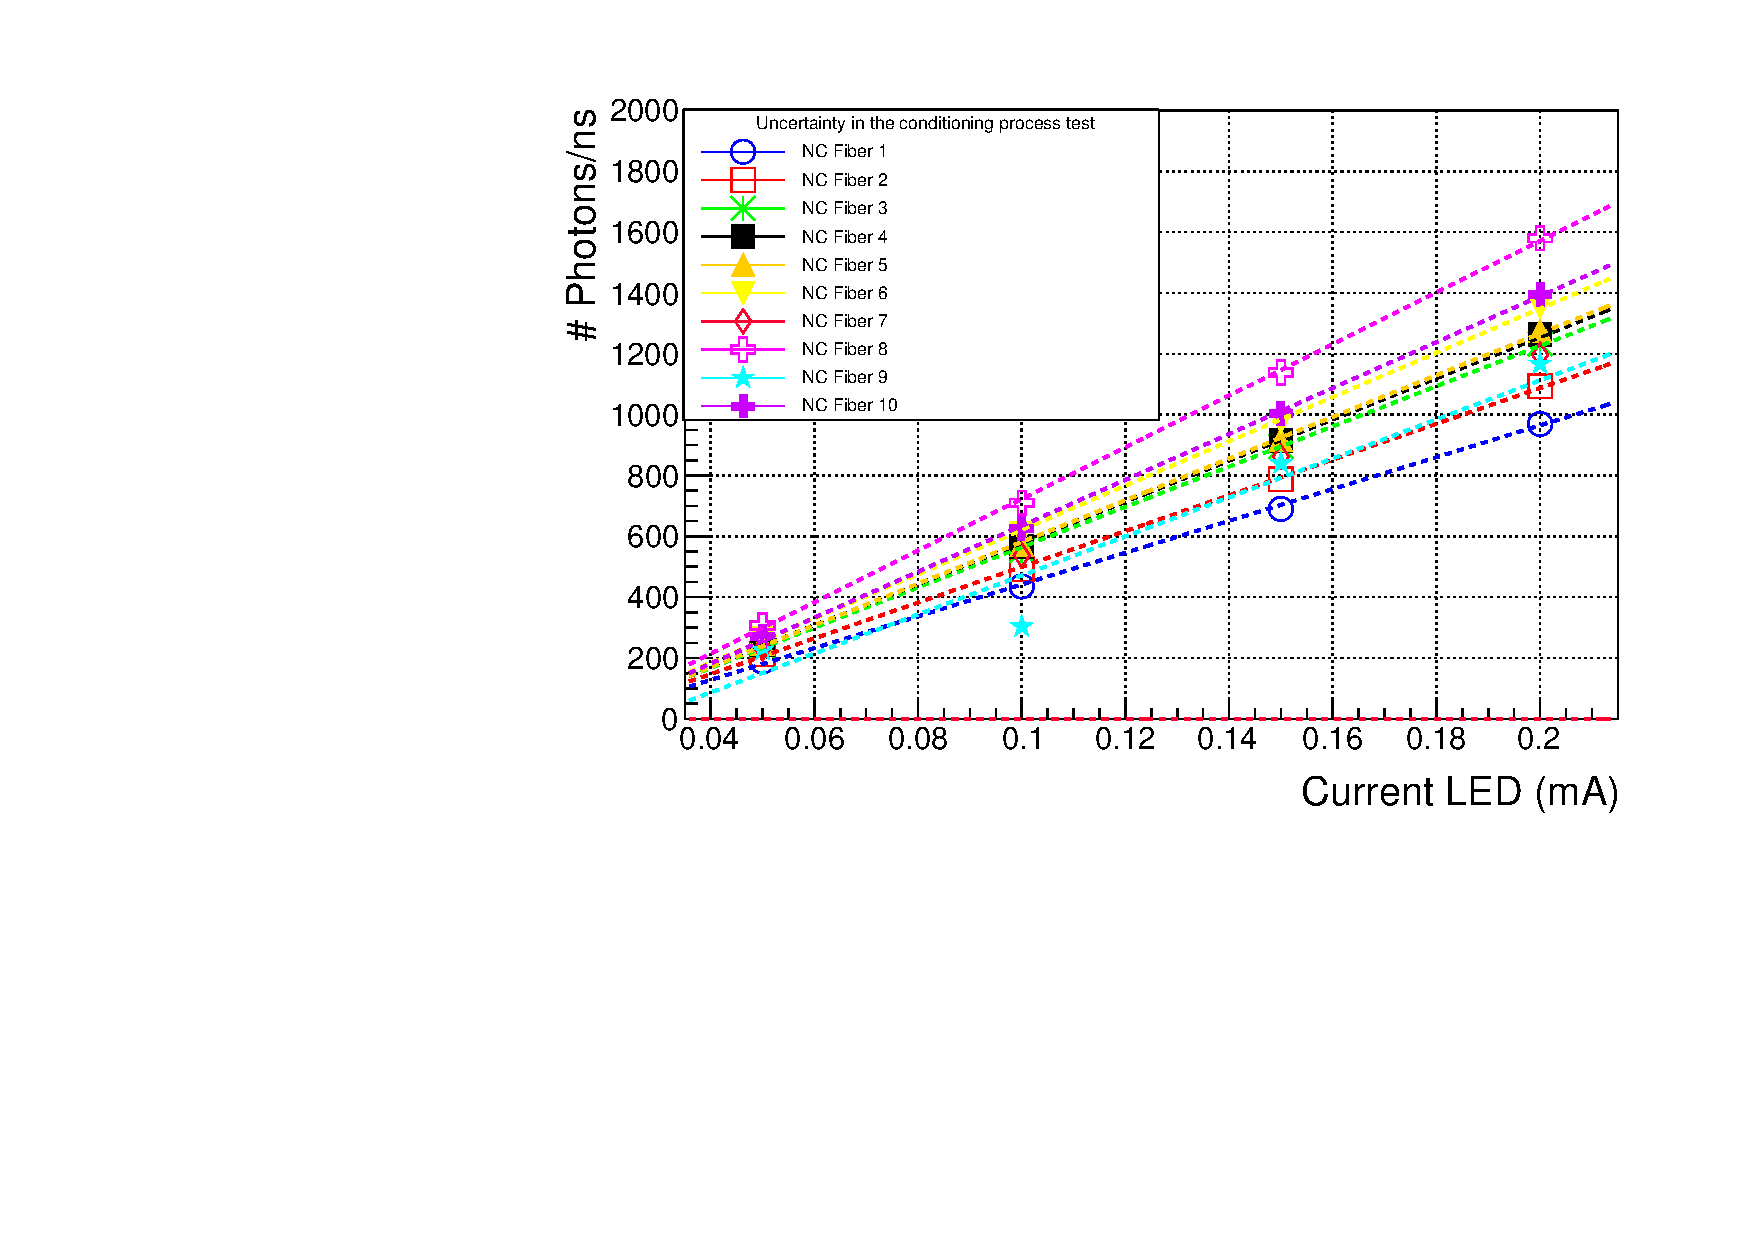
\includegraphics[scale=0.7]{4ResearchAndDevelopments/41Fibers/10_Different_samples_NoClad.pdf}
\caption{Number of photons/ns reaching the PMT for Uncladded fibers. Error bars are included but they are too small to be visible.\label{fig:10samplesNC}}
\end{figure}

\begin{figure}
\centering
    %\begin{subfigure}[b]{0.6\textwidth}
    %\centering
    %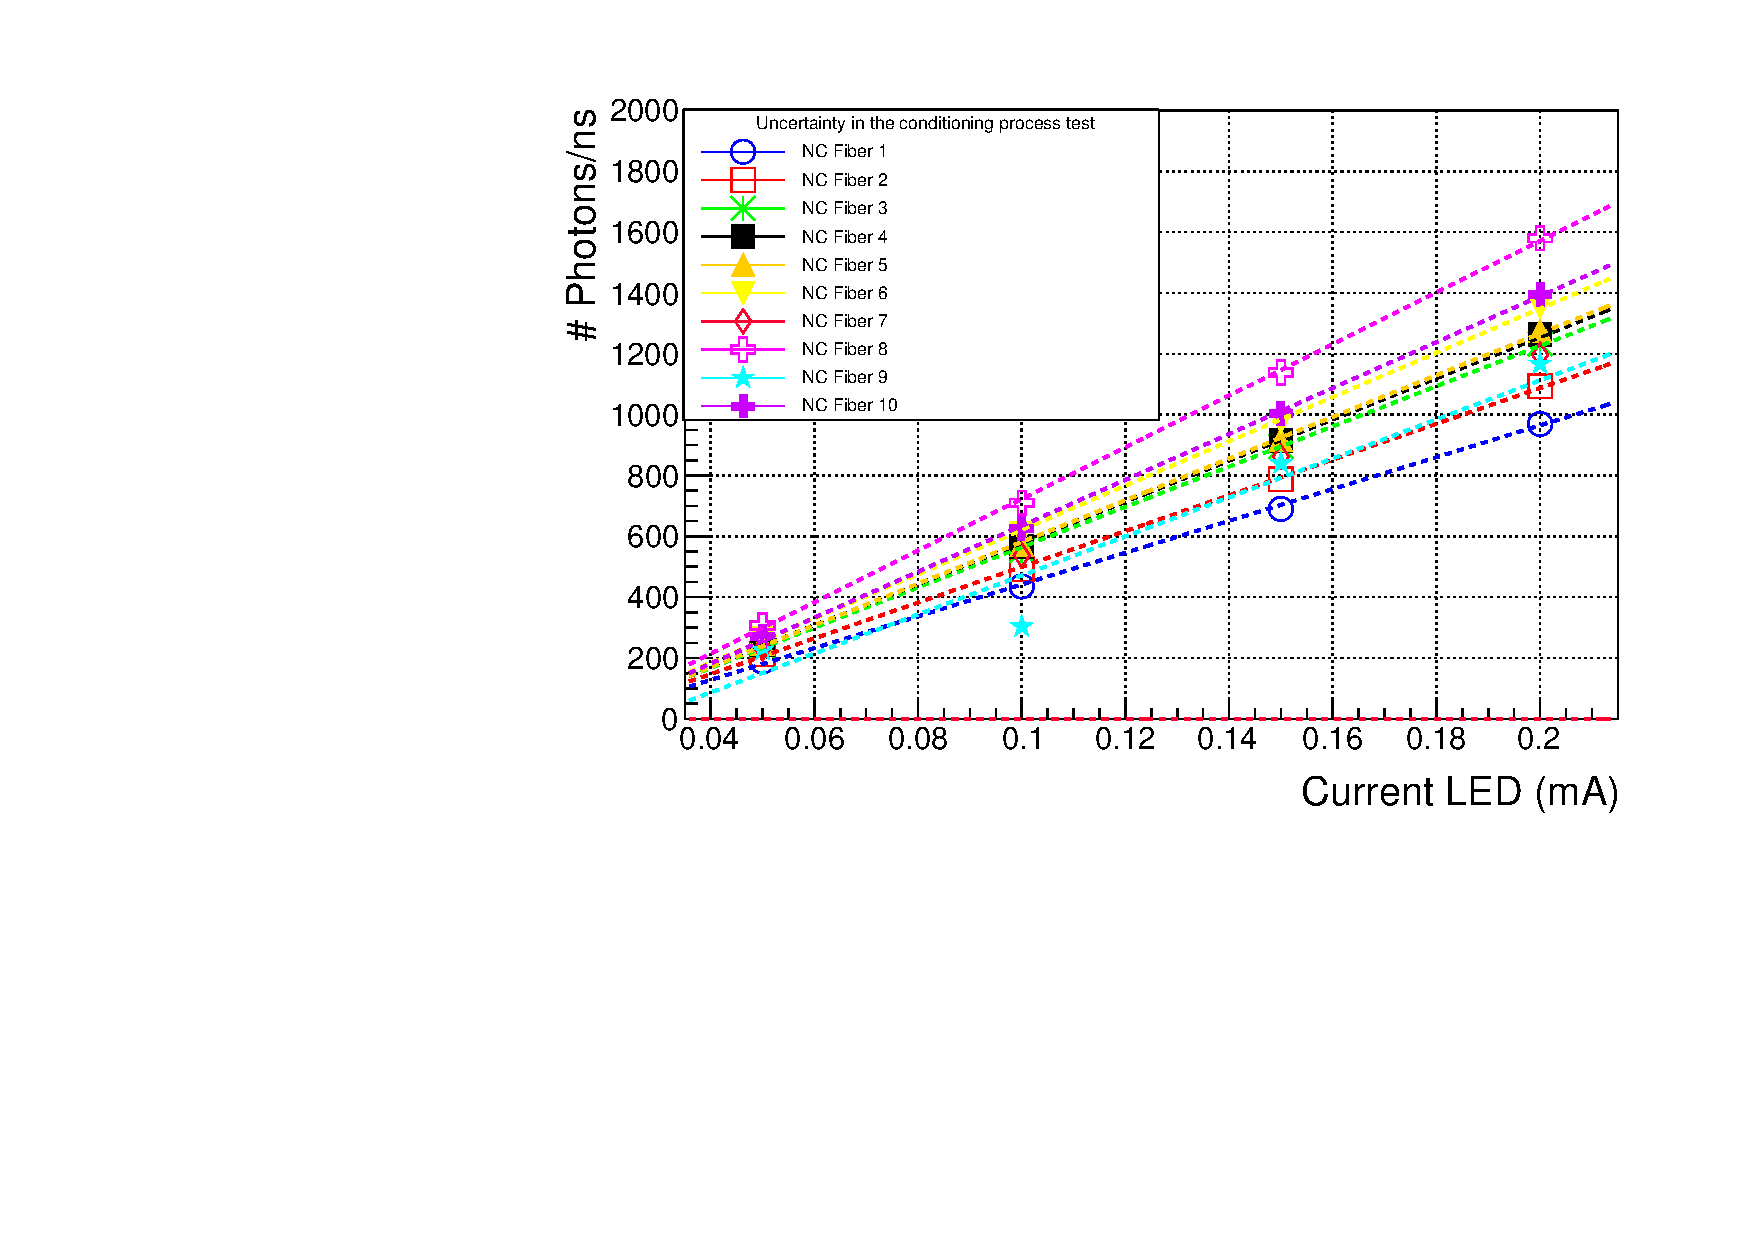
\includegraphics[width=\textwidth]{4ResearchAndDevelopments/41Fibers/10_Different_samples_NoClad.pdf}  
    %\caption{Number of photons/ns reaching the PMT for uncladded fibers.\label{subfig:10samplesNC}}
    %\end{subfigure}
    %\hfill
    \begin{subfigure}[b]{1\textwidth}
    \centering
    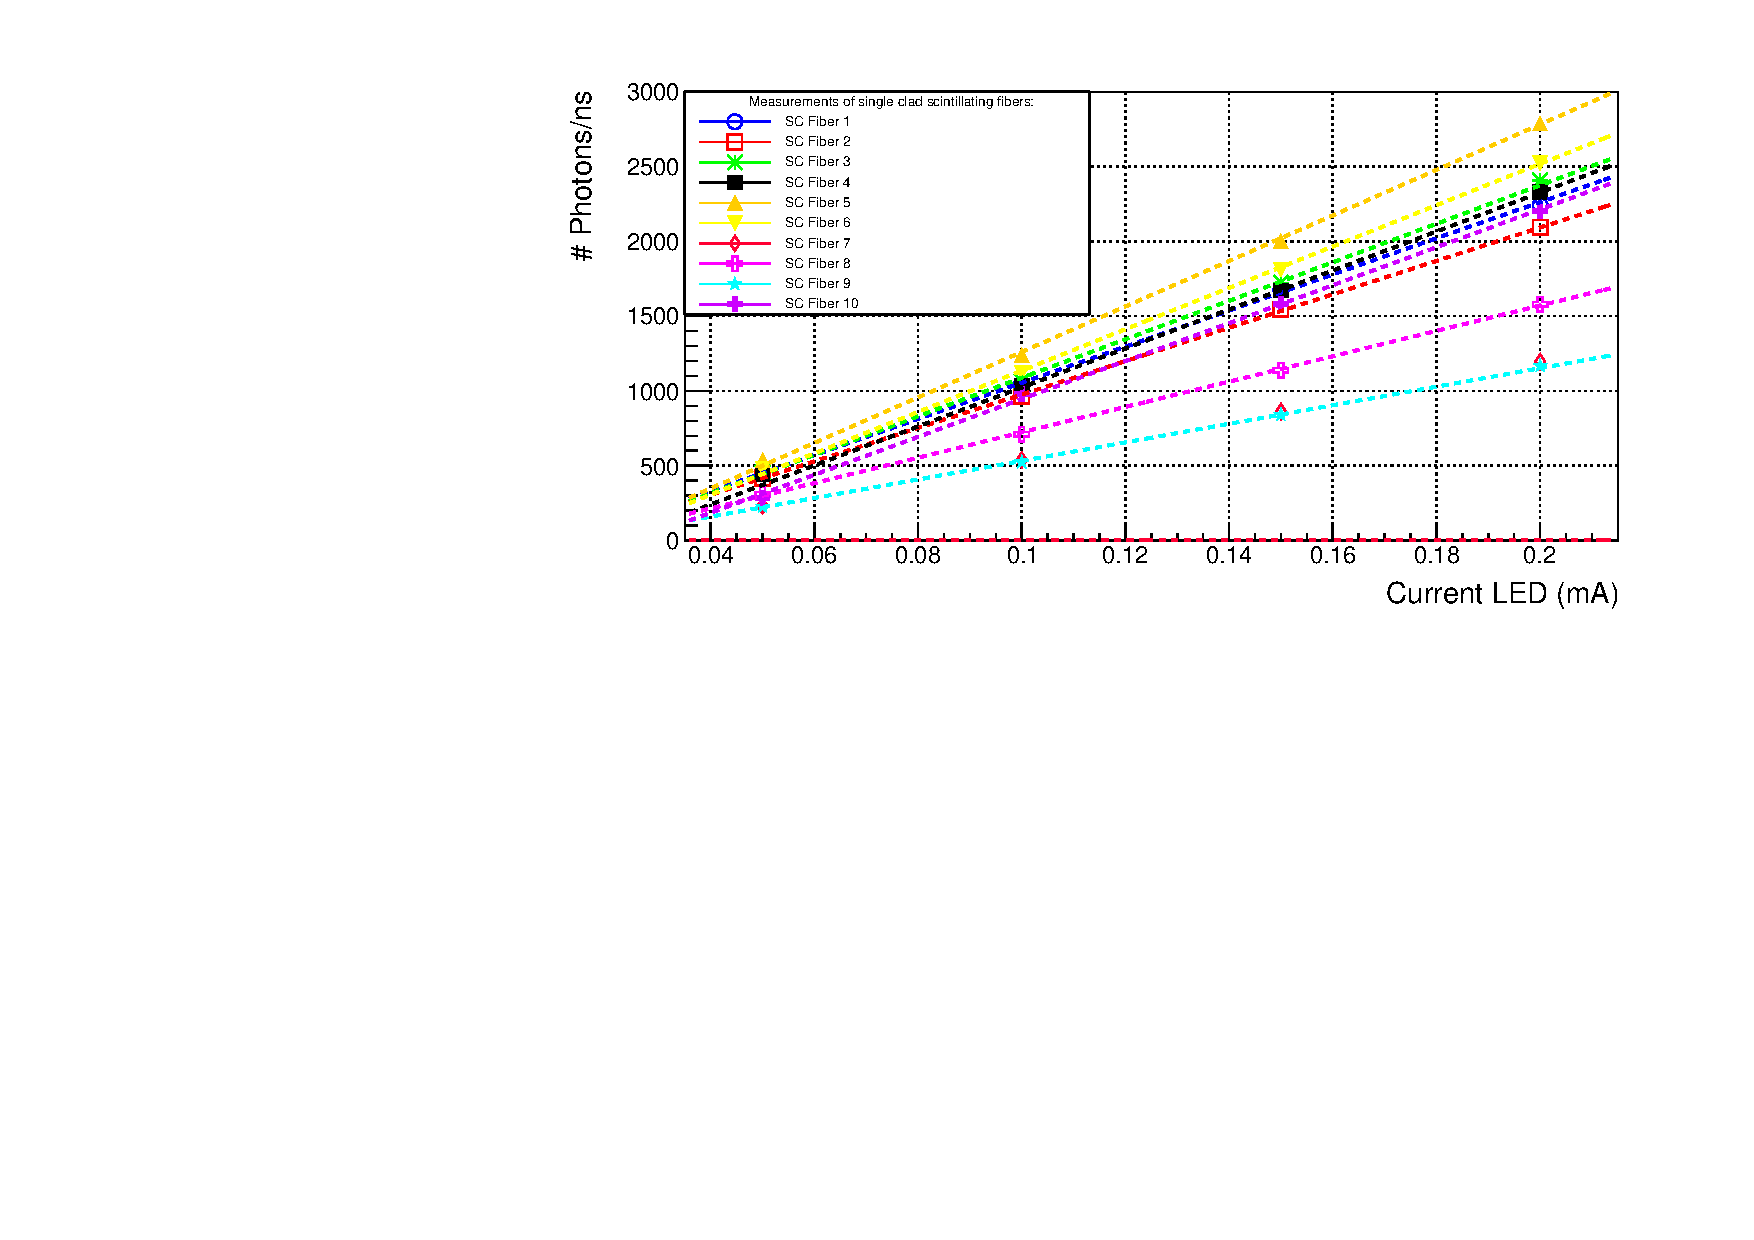
\includegraphics[width=\textwidth]{4ResearchAndDevelopments/41Fibers/10_Different_samples_SingleClad.pdf}  
    \caption{\label{subfig:10samplesSC}}
    \end{subfigure}
    \hfill
    \begin{subfigure}[b]{1\textwidth}
    \centering
    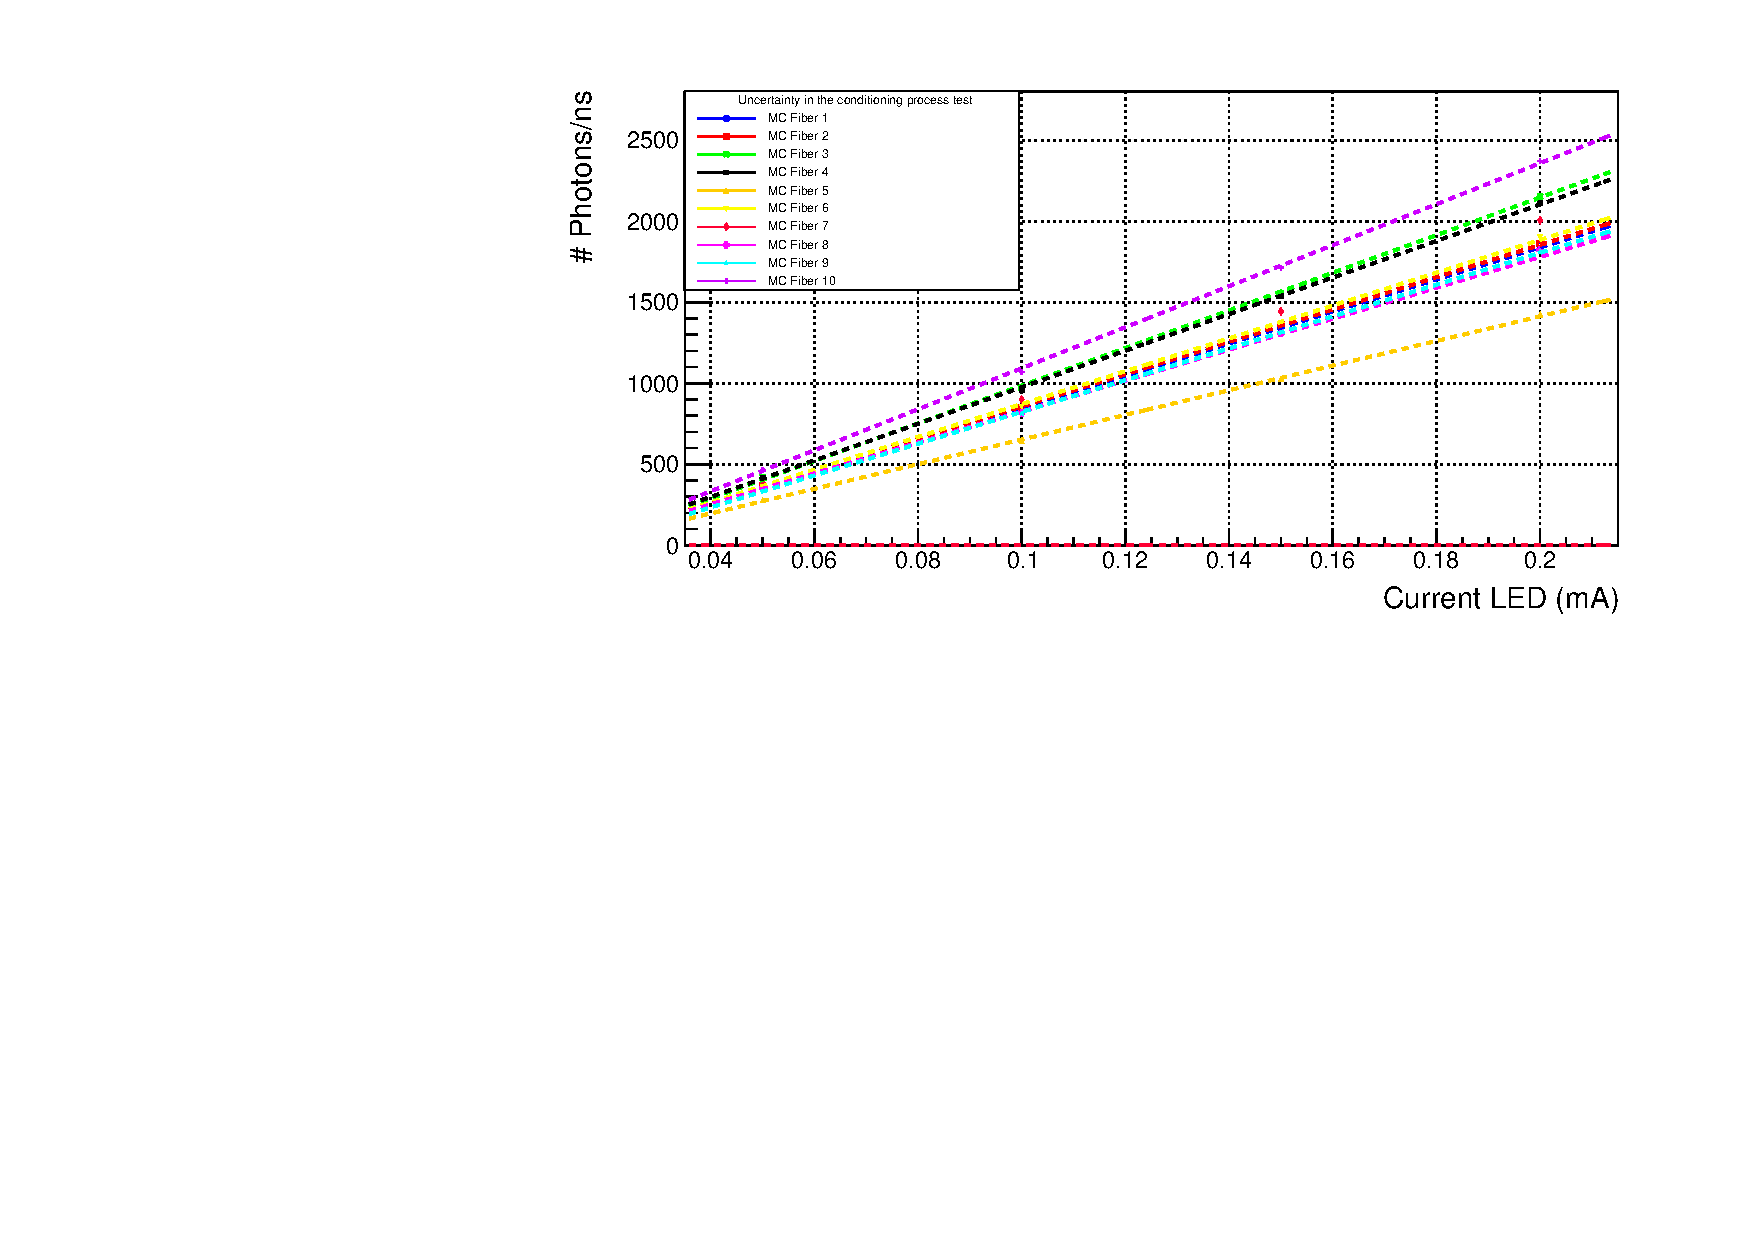
\includegraphics[width=\textwidth]{4ResearchAndDevelopments/41Fibers/10_Different_samples_MultiClad.pdf}  
    \caption{\label{subfig:10samplesMC}}
    \end{subfigure}
 \caption{Number of photons/ns reaching the PMT for ten samples of each fiber type. (Above) Single clad fibers (Below) Multi-clad fibers. Error bars are included but they are too small to be visible.}
 \label{fig:10samplesThreeTypes}
\end{figure}
The average number of collected photons versus LED intensity and the relative standard deviation for each type of fiber are given in Tables \ref{tab:10DifferentSamples} and \ref{tab:RelativeStandardDeviation3FiberTypes} respectively and are plotted in Figure \ref{fig:AveregeThreeFiberTypes}, where they can be compared. 

\begin{table}[h]
\centering{}%
\begin{tabular}{lccc}
\toprule 
Led Int. (mA) & Uncladded & Single Clad & MultiClad \tabularnewline
\midrule
\midrule 
$0.05$ & $245 \pm 11$ & $384 \pm 33$ & $377 \pm 15$ \tabularnewline
$0.1$ & $572 \pm 26$ & $923 \pm 74$ & $871 \pm 35$ \tabularnewline
$0.15$ & $915 \pm 39$ & $1485 \pm 120$ & $1397 \pm 55$ \tabularnewline
$0.2$ & $1267 \pm 55$ & $2054 \pm 166$ & $1933 \pm 76$ \tabularnewline
\bottomrule
\end{tabular}
\caption{Number of collected photons versus LED intensity for the different type of fibers.}
\label{tab:10DifferentSamples}
\end{table}

\begin{table}[h]
\centering{}%
\begin{tabular}{lccc}
\toprule 
Led Int. (mA) & Uncladded & Single Clad & MultiClad \tabularnewline
\midrule
\midrule 
$0.05$ & $4.38$ & $8.66$ & $3.97$ \tabularnewline
$0.1$ & $4.59$ & $8.02$ & $3.97$ \tabularnewline
$0.15$ & $4.34$ & $8.07$ & $3.95$ \tabularnewline
$0.2$ & $4.36$ & $8.10$ & $3.93$ \tabularnewline
Mean & $4.42$ & $8.21$ & $3.96$ \tabularnewline
\bottomrule
\end{tabular}
\caption{Relative standard deviation, $\sigma_t(\%)$, versus LED intensity for the different fiber types.}
\label{tab:RelativeStandardDeviation3FiberTypes}
\end{table}

\begin{figure}[h]
\centering
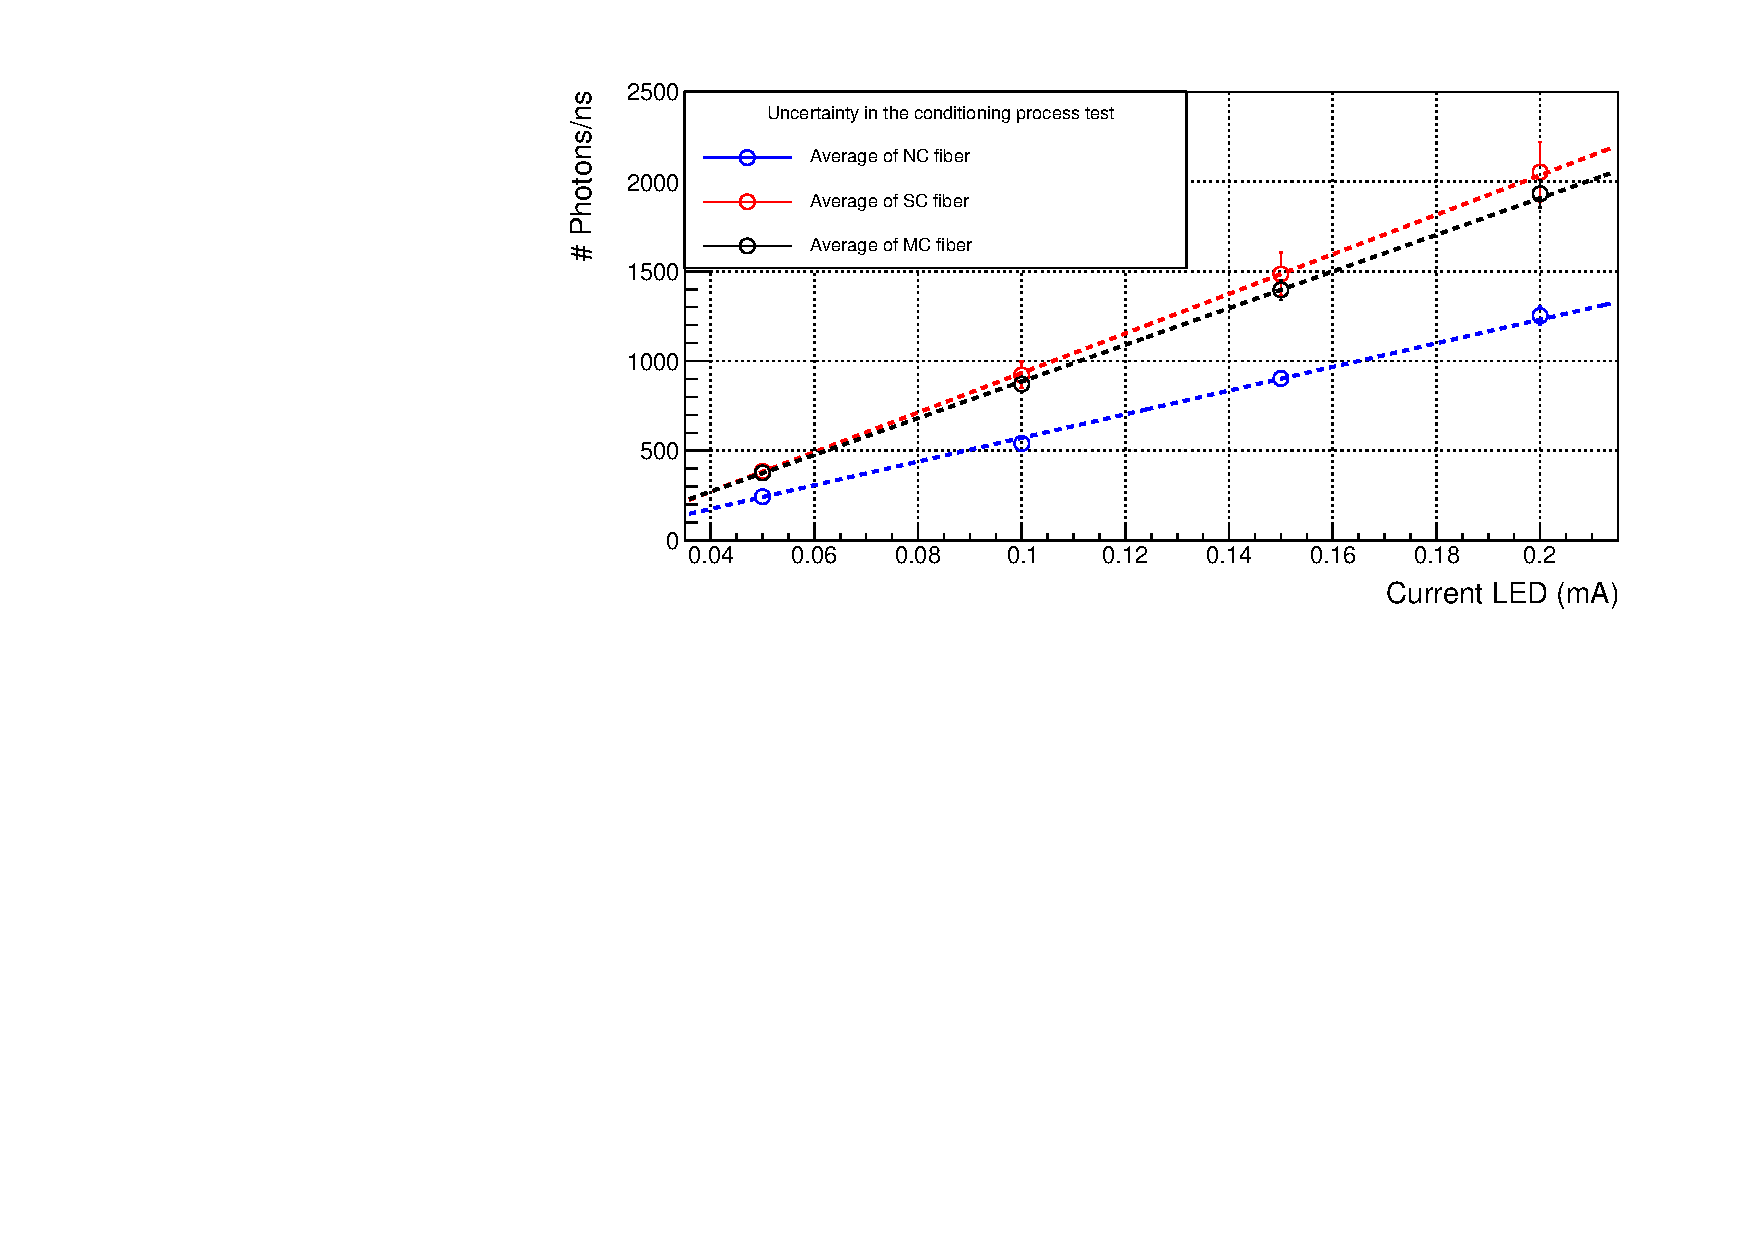
\includegraphics[scale=0.6]{4ResearchAndDevelopments/41Fibers/10_Different_Samples_Average_3_Fiber_Types.pdf}
\caption{Average number of photons versus LED current for 10 samples of each fiber type (uncladded, single clad and multi-clad fibers). Error bars are included but they are too small to be visible.\label{fig:AveregeThreeFiberTypes}}
\end{figure}

As it can be noticed in Figures \ref{fig:10samplesNC} and \ref{fig:10samplesThreeTypes} the fiber response is quite linear and single clad and multiclad fibers have stronger signals that uncladded fibers, which means that the clad has a significant effect on the fiber collection efficiency. It can also remarked in Table \ref{tab:RelativeStandardDeviation3FiberTypes} that the relative standard deviation, $\sigma^{rel}_{pos}$, does not vary with the LED intensity.

%The relative standard deviation are also presented in these tables, where we it can be seen that the dispersion of each fiber type for different LED intensities is practically negligible, which again verifies the correct behavior of the system. 

%There is only one point (uncladded fiber with $0.1~\milli\ampere $) that is higher than we expect. We can see in Table \ref{tab:10DifferentSamplesNoClad} that the reason for this is that its standard deviation is too high (as high as the measurement for uncladded fibers with $0.15~\milli\ampere$). The reason was found in the sample 9, whose measurement was very different from the average, incresing the standard deviation, probably due to a problem in the measurement process. We discard this sample because this result is not representative.

An average of the relative standard deviation caused by the fiber positioning and conditioning is given in Table \ref{tab:RelativeStandardDeviations}. As it can be noticed, the smallest relative standard deviation due to the conditioning process was found for uncladded fibers, which means that the damage from this process occurs mainly in the fiber clad, as illustrated in Figure \ref{fig:ResultofPolishingProcess}. It was checked under microscope that this damage only occurs at the end of the fiber. Also, the largest relative standard deviation in this process is measured for single clad fibers, which means that the second clad increases the resistance of the fiber to the conditioning process.

\begin{table}[htbp]
\centering{}%
\begin{tabular}{lccc}
\toprule 
Fiber type & $\sigma_t$ (\%) & $\sigma_{pos}$ (\%) & $\sigma_{con}$ (\%) \tabularnewline
\midrule
\midrule 
Uncladded & $4.42$ & $3.37$ & $2.86$ \tabularnewline
Single Clad & $8.21$ & $2.17$ & $7.92$ \tabularnewline
Multiclad & $3.96$ & $1.04$ & $3.82$ \tabularnewline
\bottomrule
\end{tabular}
\caption{Relative standard deviations ($\sigma_t$, $\sigma_{pos}$ and $\sigma_{con}$) measured in this test.}
\label{tab:RelativeStandardDeviations}
\end{table}

In summary, this study shows that the use of a fiber clad improves the photon collection efficiency. The relative statistical deviation due to the fiber conditioning process was quantified for the different fiber types. It was found that the damage by the conditioning process is produced mainly in the fiber clad. Thus, if a method to build a clad for fibers is developed, it should be applied after the fiber conditioning process.

Finally, the measurement of the photon collection efficiency for each type of fiber is shown. To measure the collection efficiency, $CE_{100}$, ten different samples $10~\cm$ length were prepared for each fiber type. Similar measurements, summarized in Table \ref{tab:10DifferentSamplesAlltypes}, were carreid out.

\begin{table}[htbp]
\centering{}%
\begin{tabular}{lccc}
\toprule 
Led Int. (mA) & Uncladded ($\gamma$/ns) & Single-clad ($\gamma$/ns) & Multi-clad ($\gamma$/ns) \tabularnewline
\midrule
\midrule 
$0.05$ & $318 \pm 61$ & $550 \pm 71$ & $480 \pm 84$ \tabularnewline
$0.1$ & $736 \pm 143$ & $1270 \pm 164$ & $1111 \pm 193$ \tabularnewline
$0.15$ & $1184 \pm 232$ & $1984 \pm 231$ & $1777\pm 307$ \tabularnewline
$0.2$ & $1645 \pm 324$ & $2507 \pm 208$ & $2338 \pm 350$ \tabularnewline
\bottomrule
\end{tabular}
\caption{Number of the collected photons versus LED intensity for 10 different fibers of $10~\cm$ length.}
\label{tab:10DifferentSamplesAlltypes}
\end{table}
The collection efficiency of $10~\cm$ fiber length, $CE_{10}$, was calculated by comparing these tests to those performed for a fiber length of $20~\cm$. The collection efficiency  to $CE_{100}$ was calculated from $CE_{10}$ by assuming a linear dependence on length.

\begin{table}[htbp]
\centering{}%
\begin{tabular}{lcc}
\toprule 
Fiber type & $CE_{10}$ (\%) & $CE_{100}$ (\%) \tabularnewline
\midrule
\midrule 
UnCladded & $76 \pm 8$ & $7.6 \pm 0.8$ \tabularnewline
Single Clad & $78 \pm 6$ & $7.8 \pm 0.6$ \tabularnewline
Multiclad & $83 \pm 7$ & $8.3 \pm 0.7$ \tabularnewline
\bottomrule
\end{tabular}
\caption{Collection efficiencies $CE_{10}$ and $CE_{100}$.}
\label{tab:CollectionEfficiencyOfFibers}
\end{table}
The collection efficiency, $CE_{100}$, given by the manufacturer Saint-Gobain is in the range $3.44\%-7\%$ \cite{DataSheetBCF12Fiber}. Our measurements, given in Table \ref{tab:CollectionEfficiencyOfFibers}, are close but slightly higher than the manufacturer values which could be attributed to our use of collimated photons.

%As collimated photons were used in this study, the fact that our results are in the best side is justified. As it can be seen in Table \ref{tab:CollectionEfficiencyOfFibers}, our measured values are very close to those provided by the manufacturer. %The difference between this value for the three types of fiber studied is not as large as it was expected. A possible reason is that the difference in fiber length is only $10~\cm$ and it may not be enough to see this effect. It could be interesting to repeat these tests with a larger difference in fiber length.